\documentclass[11pt]{standalone}

\usepackage{amssymb} 
\usepackage{amsmath} 

\usepackage[no-math]{fontspec}
\usepackage{unicode-math}
\setmainfont{Lato}
\setmathfont{Stix Two Math}

\usepackage{tikz}
\usetikzlibrary{arrows.meta}
\usepackage{pgfplots}
\pgfplotsset{compat=newest}
\usetikzlibrary{backgrounds}

\usepackage{xcolor}
\definecolor{accent1}{RGB}{0,90,148}
\definecolor{accent2}{RGB}{204,222,233}
\definecolor{alert}{RGB}{230,0,0}
\definecolor{bg}{RGB}{243,244,244}
\definecolor{fg}{RGB}{72,73,73}


\makeatletter
\tikzset{fixed ratio/.code={\def\tikz@pft##1:##2;{\edef\pgfutil@tempx{##1}\edef\pgfutil@tempy{##2}}%
    \expandafter\tikz@pft#1;%
    \tikzset{execute at end picture={%
    \ifcsname sa@border@right\endcsname
     \pgfmathsetmacro\pgfutil@tempa{((\pgf@picmaxx+\sa@border@right-\pgf@picminx+\sa@border@left)/%
     (\pgf@picmaxy+\sa@border@top-\pgf@picminy+\sa@border@bottom)}%
    \else
     \pgfmathsetmacro\pgfutil@tempa{((\pgf@picmaxx-\pgf@picminx)/(\pgf@picmaxy-\pgf@picminy)}%
    \fi
    \pgfmathsetmacro\pgfutil@tempb{(\pgfutil@tempx/\pgfutil@tempy)}%
    \ifdim\pgfutil@tempa pt=\pgfutil@tempb pt\relax
    \else
     \ifdim\pgfutil@tempb pt>\pgfutil@tempa pt\relax
      % target ratio greater than actual
      \pgfmathsetmacro\pgfutil@tempc{-(\pgf@picmaxx-\pgf@picminx)%
      +\pgfutil@tempb*(\pgf@picmaxy-\pgf@picminy)}%
      \path ([xshift=-0.5*\pgfutil@tempc]current bounding box.west)
       ([xshift=0.5*\pgfutil@tempc]current bounding box.east);
     \else
      % target ratio smaller than actual
      \pgfmathsetmacro\pgfutil@tempc{-(\pgf@picmaxy-\pgf@picminy)%
      +(\pgf@picmaxx-\pgf@picminx)/\pgfutil@tempb}%
      \path ([yshift=-0.5*\pgfutil@tempc]current bounding box.south)
       ([yshift=0.5*\pgfutil@tempc]current bounding box.north);
     \fi
    \fi
    }%  
    }}
}
\makeatother



\usetikzlibrary{datavisualization.polar, datavisualization.formats.functions}
\usepgfplotslibrary{polar}

\begin{document}
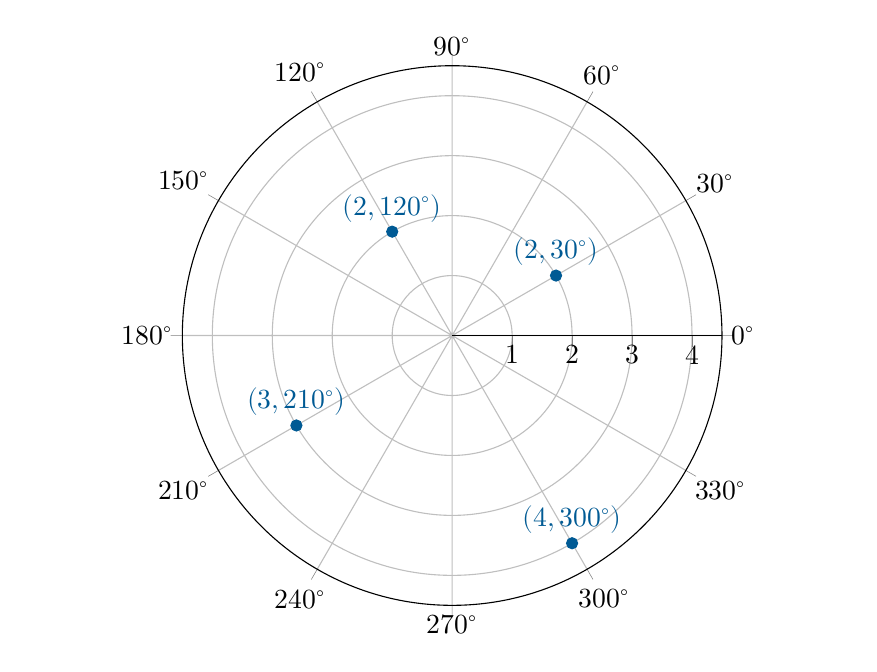
\begin{tikzpicture}[fixed ratio=4:3]
\begin{polaraxis}[
    % Polar axis configuration
    clip=false,
    xmin=0, xmax=360,
    ymin=0, ymax=4.5,
    xtick={0,30,...,330},
    ytick={1,2,3,4},
    xticklabels={$0^\circ$,$30^\circ$,$60^\circ$,$90^\circ$,
    	$120^\circ$,$150^\circ$,$180^\circ$,$210^\circ$,$240^\circ$,
	    $270^\circ$,$300^\circ$,$330^\circ$},
    yticklabels={1,2,3,4},
    grid=both,
    major grid style={solid},
    ytick align=outside,
    yticklabel style={anchor=north, yshift=-\pgfkeysvalueof{/pgfplots/major tick length}}
]
% Add points
\addplot+[mark=*, 
	mark options={fill=accent1, draw=accent1}, nodes near coords, only marks, 
	point meta=explicit symbolic, color=accent1] 
	coordinates {
    (30,2)[$(2,30^\circ)$]
    (120,2)[$(2,120^\circ)$]
    (210,3)[$(3,210^\circ)$]
    (300,4)[$(4,300^\circ)$]
};
\end{polaraxis}
\end{tikzpicture}
\end{document}